\documentclass[12pt]{article}
\usepackage{fullpage}

\usepackage[T1]{fontenc}
\usepackage[utf8]{inputenc}
\usepackage{lmodern}
\usepackage{microtype}
\usepackage[full]{textcomp}
\usepackage[osf]{newtxtext}
\usepackage{graphicx}

%% ---- Base math packages (always available) -------------------------------
\usepackage{amsmath, amssymb, amsthm, mathtools}
\usepackage{hyperref}

%% ---- Submission preamble (imported so the inlined solution compiles) ----
\usepackage{amsmath,amssymb,amsthm}

\newtheorem{theorem}{Theorem}
\newtheorem{lemma}{Lemma}
\newtheorem{proposition}{Proposition}

\newcommand{\Aut}{\operatorname{Aut}}
\newcommand{\dom}{\operatorname{dom}}

%% ---- Theorem environments not supplied by the submission ------------------
\makeatletter
\@ifundefined{theorem}{\newtheorem{theorem}{Theorem}}{}
\@ifundefined{lemma}{\newtheorem{lemma}{Lemma}}{}
\@ifundefined{proposition}{\newtheorem{proposition}{Proposition}}{}
\@ifundefined{corollary}{\newtheorem{corollary}{Corollary}}{}
\@ifundefined{definition}{\theoremstyle{definition}\newtheorem{definition}{Definition}}{}
\@ifundefined{remark}{\theoremstyle{remark}\newtheorem{remark}{Remark}}{}
\makeatother

%% ---- First Proof theme + in-text comment box -----------------------------
%% Palette from the FINAL DELIVERABLES brand assets:
%%   slate     #171313  (ink)
%%   warm-gray #69626D  (secondary)
%%   sand      #F2ECE9  (light background)
\usepackage{xcolor}
\usepackage[most]{tcolorbox}

\definecolor{FPslate}{HTML}{171313}
\definecolor{FPwarmgray}{HTML}{69626D}
\definecolor{FPsand}{HTML}{F2ECE9}

% Reviewer number for this document (set per file). Used by the comment box tag.
\newcommand{\reviewernum}{2}

% \review{...} : a First-Proof-themed reviewer comment, set inline in the text
%            as a sand box with a warm-gray rule and a "Reviewer N" tag.
\newtcolorbox{reviewbox}{
  breakable, enhanced, sharp corners,
  colback=FPsand, colframe=FPwarmgray,
  coltext=FPslate, boxrule=0pt, leftrule=2.5pt,
  left=8pt, right=8pt, top=14pt, bottom=5pt,
  before skip=6pt, after skip=6pt,
  fontupper=\small,
  overlay unbroken and first={
    \node[anchor=north east, font=\bfseries\footnotesize\sffamily,
          text=FPwarmgray, inner sep=0pt]
      at ([xshift=-8pt,yshift=-4pt]frame.north east) {Reviewer~\reviewernum};}
}
\newcommand{\review}[1]{\begin{reviewbox}#1\end{reviewbox}}

\title{Review of Submission 1C}
\author{First Proof Second Batch \\ Reviewer \reviewernum}
\date{June 4--8, 2026}

\makeatletter
\renewcommand{\maketitle}{%
  \noindent
  \begin{minipage}[t]{0.68\textwidth}
    \vspace{20pt}
    \raggedright
    {\LARGE\bfseries \@title\par}
    \vspace{0.35em}
    {\large \@author\par}
    \vspace{0.35em}
    {\normalsize \@date\par}
  \end{minipage}%
  \hfill
  \begin{minipage}[t]{0.25\textwidth}
    \vspace{0pt}
    \raggedleft
    \raisebox{\dimexpr-\height+\ht\strutbox+0.225in\relax}{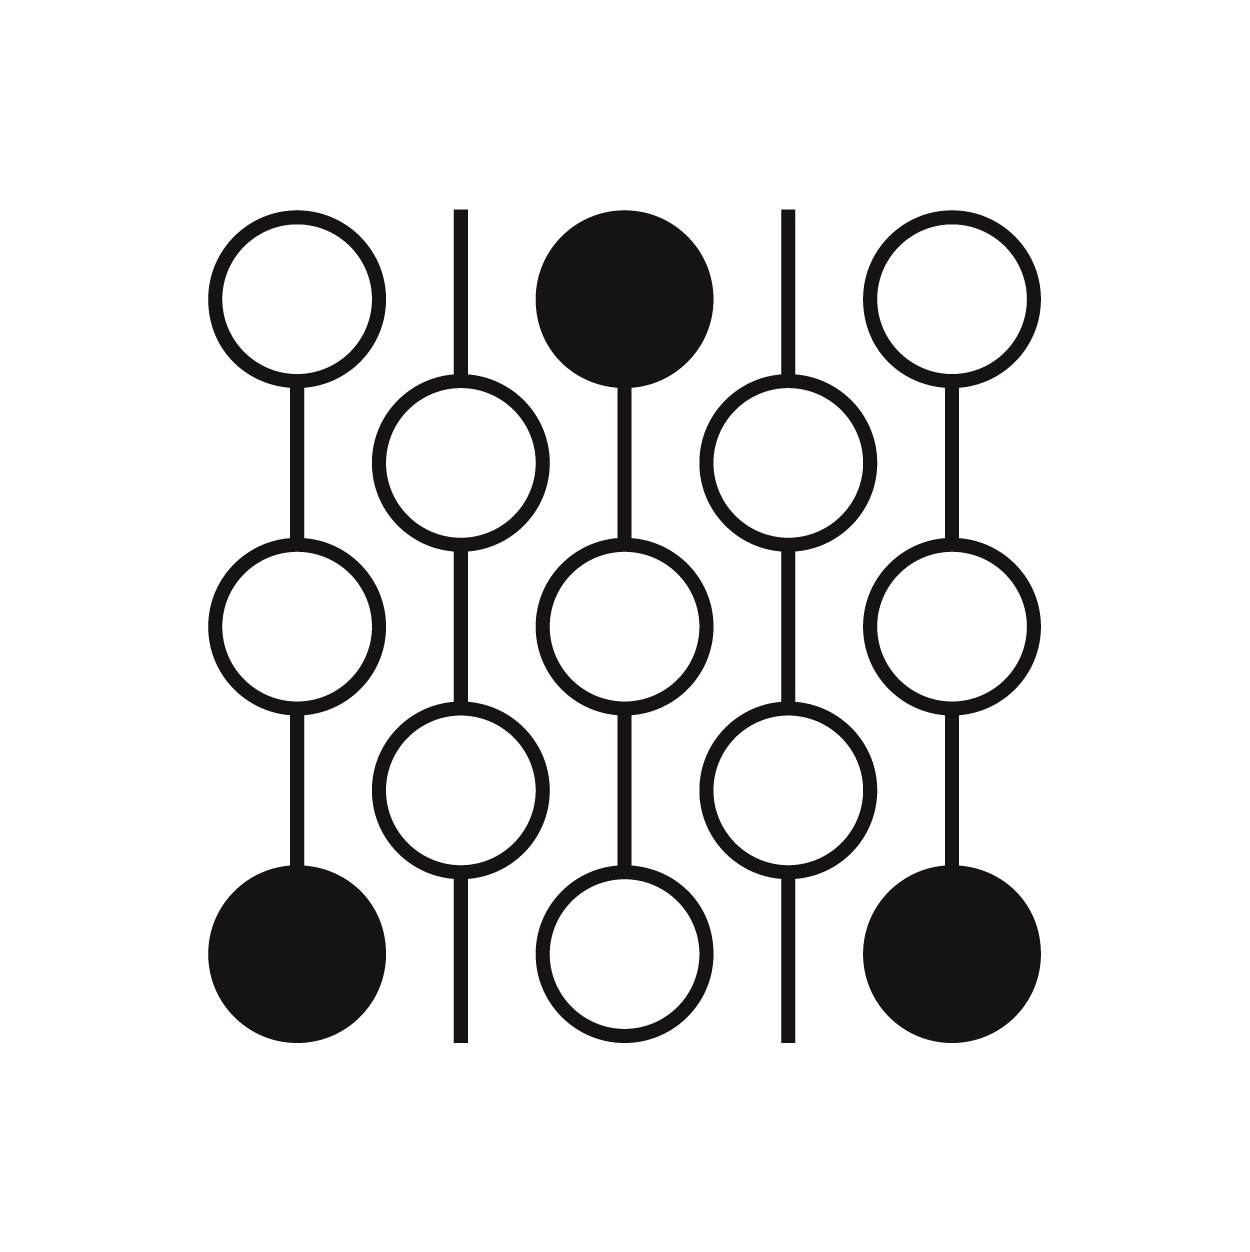
\includegraphics[height=1.35in]{Logo-slate.png}}
  \end{minipage}
  \par\vspace{2em}
}
\makeatother

\begin{document}
\maketitle
\section{Review}


\paragraph{Correctness.}

Problem 1 asks whether there exists a computable structure with certain properties, and this submission correctly constructs an example of such a structure. The structure $\mathcal{A}$ constructed is in a countably infinite language consisting of infinitely many unary and binary relation symbols and one unary function symbol. The proof characterizes the automorphisms of $\mathcal{A}$ by associating each $\alpha \in \mathcal{A}$ to a finite set $g \in [\omega]^{< \omega}$. Finally, it verifies the construction by checking that $\mathcal{A}$ indeed satisfies the required properties. The level of detail in the proof matches the expected level of detail from a journal paper.

\paragraph{Novelty.} The proof uses standard techniques from computability theory and computable structure theory. In the opinion of this reviewer, there is no evidence that the solution is following a similar proof from another source. This submission is most similar to Submission B, though Submission C uses an infinite language unlike Submission B's finite relational language. The infinite language makes the construction somewhat cleaner. This submission is less similar to Submission A or the human solution.

\paragraph{Attribution} The submission makes no attributions. While this submission does not closely follow or adapt an existing argument, there are somewhat similar arguments in the literature, and those should be cited, such as the following:
\begin{itemize}
    \item Coding in the Automorphism Group of a Computably Categorical Structure, by Turetsky
    \item Degrees of Categoricity and Treeable Degrees, by Csima and Rossegger
    \item Scott Complexity of Countable Structures, by Alvir, Greenberg, Harrison-Trainor, and Turetsky
\end{itemize}

\section{Recommendation}

The submission is \textbf{publishable with minor revisions}. As stated above, the proof is correct and contains no inaccuracies. The in-text comments below are mostly stylistic disagreements. Additionally, the techniques in the paper are just similar enough to the techniques in other papers that should be mentioned and cited, even if the argument in this submission does not exactly follow any existing, published argument.

  \section{Submission with inline comments}

%% ======================================================================
%% Inlined verbatim from the anonymised submission prob_001-C.
%% ======================================================================

\date{}



\begin{abstract}
We answer the question affirmatively.  We build a computable countable
structure $\mathcal A$ such that every automorphism of every copy of
$\mathcal A$ is computable from that copy, but for every finite tuple of
parameters $\bar a$ there is an automorphism $\pi$ whose graph is not
$\Sigma^{\mathrm{in}}_1$-definable over $\bar a\cup\pi(\bar a)$.
\end{abstract}

\subsection*{The construction}

Let
\[
G=[\omega]^{<\omega}
\]
be the countable Boolean group of finite subsets of $\omega$, with operation
symmetric difference $\triangle$.  For $g\in G$ and $n\in\omega$, write
\[
\epsilon_n(g)=
\begin{cases}
1,& n\in g,\\
0,& n\notin g.
\end{cases}
\]
Let $e_n=\{n\}$.

We use a computable countable language $L$ containing:
\begin{itemize}
\item unary predicates $U,V_0,V_1,\dots$;
\item for each $g\in G$, a binary relation symbol $Q_g$;
\item for each $n\in\omega$, a binary relation symbol $P_n$;
\item one unary function symbol $S$.
\end{itemize}

\review{The structure is in an infinite language, whereas Submission B and the human solution build structures in finite languages. This difference is mostly stylistic but perhaps worth noting. The infinite language does simplify the construction.}

The domain of $\mathcal A$ is the disjoint union
\[
U^{\mathcal A}\ \cup\ \bigcup_{n\in\omega}V_n^{\mathcal A},
\]
where
\[
U^{\mathcal A}=G
\]
and
\[
V_n^{\mathcal A}=V_n^0\cup V_n^1,\qquad
V_n^i=\{v_{n,i,m}:m\in\omega\}.
\]
The predicates $U,V_n$ name these sorts.  The symbols are interpreted as follows:
\[
Q_g(u,v)\quad\Longleftrightarrow\quad u,v\in U^{\mathcal A}
\ \text{ and }\ v=u\triangle g;
\]
\[
P_n(u,v_{n,i,m})\quad\Longleftrightarrow\quad
u\in U^{\mathcal A}\ \text{ and }\ i=\epsilon_n(u),
\]
and $P_n$ is false outside $U^{\mathcal A}\times V_n^{\mathcal A}$.  Finally,
\[
S(u)=u\quad(u\in U^{\mathcal A}),
\]
and
\[
S(v_{n,i,m})=v_{n,i,m+1}.
\]
With any standard computable coding of $G$ and of the triples $(n,i,m)$, this is a computable presentation of $\mathcal A$.

\subsection*{The automorphism group}

For each $g\in G$, define a permutation $\tau_g$ of $\mathcal A$ by
\[
\tau_g(u)=g\triangle u\qquad(u\in U^{\mathcal A}),
\]
and
\[
\tau_g(v_{n,i,m})=v_{n,i\oplus \epsilon_n(g),m}.
\]
Here $\oplus$ denotes addition modulo $2$.

\begin{lemma}
For every $g\in G$, $\tau_g\in\Aut(\mathcal A)$, and every automorphism of
$\mathcal A$ is of this form.  Hence
\[
\Aut(\mathcal A)=\{\tau_g:g\in G\}\cong G
\]
is countable.
\end{lemma}

\begin{proof}
It is immediate from the definitions that $\tau_g$ preserves all sort predicates and preserves $S$.

\review{Indeed, it is appropriate at this level to not need to check with great detail that $\tau_g$ preserves those relations.}

If $Q_h(u,v)$ holds, then $v=u\triangle h$, and therefore
\[
\tau_g(v)=g\triangle u\triangle h=\tau_g(u)\triangle h,
\]
so $Q_h(\tau_g(u),\tau_g(v))$ holds.

Similarly, if $P_n(u,v_{n,i,m})$ holds, then $i=\epsilon_n(u)$.  Since
\[
\epsilon_n(g\triangle u)=\epsilon_n(g)\oplus\epsilon_n(u),
\]
we have
\[
P_n(\tau_g(u),\tau_g(v_{n,i,m})).
\]
Thus $\tau_g$ is an automorphism.

Conversely, let $\alpha\in\Aut(\mathcal A)$.  Since $U$ is named, $\alpha$ maps $U^{\mathcal A}$ to itself.  Put
\[
g=\alpha(\varnothing)\in G.
\]
For every $u\in G$, the relation $Q_u(\varnothing,u)$ holds.  Applying $\alpha$, we get
\[
Q_u(g,\alpha(u)),
\]
so
\[
\alpha(u)=g\triangle u.
\]

Now fix $n$ and consider $V_n$.  Let $v=v_{n,i,m}$.  Choose $u\in G$ with
$\epsilon_n(u)=i$.  Then $P_n(u,v)$ holds.  Applying $\alpha$, we get
\[
P_n(g\triangle u,\alpha(v)).
\]
Therefore $\alpha(v)$ lies in the copy $V_n^{i\oplus\epsilon_n(g)}$.

Finally, $\alpha$ preserves $S$.  On each copy $V_n^i$, the map $S$ is the successor map on a one-way chain of type $\omega$.  Any bijection between two such chains preserving successor must send the unique element not in the range of $S$ to the unique element not in the range of $S$, and hence must preserve the coordinate $m$.  Thus
\[
\alpha(v_{n,i,m})=v_{n,i\oplus\epsilon_n(g),m}.
\]
So $\alpha=\tau_g$.
\end{proof}

\review{Compare to Lemmas 3.5 and 3.6 of Submission B.}

\subsection*{Every automorphism of every copy is relatively computable}

\begin{proposition}
For every copy $\mathcal B\cong\mathcal A$ and every
$\beta\in\Aut(\mathcal B)$, the function $\beta$ is computable relative to
the atomic diagram of $\mathcal B$.  In particular, $\mathcal A$ is
computably $\Aut$-countable on the cone with base $\emptyset$.
\end{proposition}

\begin{proof}
Let $\mathcal B$ be any copy of $\mathcal A$, and let
$\beta\in\Aut(\mathcal B)$.  By the previous lemma, transferred to
$\mathcal B$, there is a unique $g\in G$ such that $\beta$ acts on the $U$-sort as translation by $g$.  Since $g$ is a finite subset of $\omega$, it can be hard-coded into a Turing program computing $\beta$.

Choose any $u_0\in U^{\mathcal B}$ and let
\[
u_1=\beta(u_0).
\]
The program may hard-code the natural numbers $u_0,u_1$.

Given input $x\in U^{\mathcal B}$, search through $h\in G$ until finding the unique $h$ such that
\[
\mathcal B\models Q_h(u_0,x).
\]
Then search for the unique $y$ such that
\[
\mathcal B\models Q_h(u_1,y).
\]
Output this $y$.  This computes $\beta(x)$ for $x\in U^{\mathcal B}$.

Now suppose $x\in V_n^{\mathcal B}$.  We can find $n$ by searching the unary predicates $V_0,V_1,\dots$.

If $n\notin g$, then $\beta$ is the identity on $V_n^{\mathcal B}$, so output $x$.

If $n\in g$, then $\beta$ swaps the two $S$-chains inside $V_n^{\mathcal B}$.  Choose some
\[
p_n\in V_n^{\mathcal B}
\]
and let
\[
q_n=\beta(p_n).
\]
The program may hard-code the finitely many pairs $(p_n,q_n)$ for $n\in g$.

To compute $\beta(x)$ for $x\in V_n^{\mathcal B}$ with $n\in g$, dovetail the following searches:
\begin{itemize}
\item search for $d$ with $S^d(p_n)=x$; if found, output $S^d(q_n)$;
\item search for $d$ with $S^d(x)=p_n$; if found, search for the unique $y$ with $S^d(y)=q_n$, and output $y$;
\item search for $d$ with $S^d(q_n)=x$; if found, output $S^d(p_n)$;
\item search for $d$ with $S^d(x)=q_n$; if found, search for the unique $y$ with $S^d(y)=p_n$, and output $y$.
\end{itemize}
Exactly one of these alternatives eventually applies, because each $V_n$ consists of two one-way $S$-chains and $p_n,q_n$ are corresponding points in the two chains.

All searches use only the atomic diagram of $\mathcal B$.  Thus $\beta$ is computable relative to $\mathcal B$.

\review{There are some unnecessary details in this proof but no inaccuracies.}

\end{proof}

\subsection*{A preservation lemma for existential formulas}

Fix $n$.  For $d_0,d_1\in\omega$, define a map
\[
\rho^{n}_{d_0,d_1}:\mathcal A\to\mathcal A
\]
by fixing every element outside $V_n$, and by
\[
\rho^{n}_{d_0,d_1}(v_{n,i,m})=v_{n,i,m+d_i}.
\]

\begin{lemma}
For every $n$ and every $d_0,d_1\in\omega$, the map
$\rho^{n}_{d_0,d_1}$ is an embedding of $\mathcal A$ into itself.
Consequently, if an existential formula with parameters outside $V_n$
holds of a tuple, then it still holds after applying $\rho^{n}_{d_0,d_1}$
to the non-parameter entries.
\end{lemma}

\begin{proof}
The map $\rho^{n}_{d_0,d_1}$ is injective.  It clearly preserves the unary predicates.  It fixes $U$, so it preserves every $Q_g$.  It also preserves $S$, because
\[
\rho^{n}_{d_0,d_1}(S(v_{n,i,m}))
=
v_{n,i,m+1+d_i}
=
S(\rho^{n}_{d_0,d_1}(v_{n,i,m})).
\]
Finally, $P_n(u,v_{n,i,m})$ depends only on $u$ and on the copy index $i$, and $\rho^{n}_{d_0,d_1}$ fixes $u$ and preserves $i$.  For $m\neq n$, $P_m$ is unaffected.

Thus $\rho^{n}_{d_0,d_1}$ is an $L$-embedding.  Embeddings preserve quantifier-free formulas, and therefore preserve existential formulas.
\end{proof}

\subsection*{Failure of $\Sigma^{\mathrm{in}}_1$-definability}

\begin{lemma}
Let $\bar p$ be a finite tuple from $\mathcal A$ containing no element of
$V_n$.  Then the automorphism $\tau_{e_n}$ is not
$\Sigma^{\mathrm{in}}_1$-definable over $\bar p$.
\end{lemma}

\begin{proof}
Let
\[
r_0=v_{n,0,0},\qquad r_1=v_{n,1,0}.
\]
Then
\[
\tau_{e_n}(r_0)=r_1.
\]

Suppose, toward a contradiction, that the graph of $\tau_{e_n}$ is
$\Sigma^{\mathrm{in}}_1$-definable over $\bar p$.  Then there is a countable
family of existential formulas
\[
(\varphi_i(\bar p,x,y))_{i\in\omega}
\]
such that
\[
\tau_{e_n}(x)=y
\quad\Longleftrightarrow\quad
\mathcal A\models \varphi_i(\bar p,x,y)
\ \text{ for some }i.
\]
Since $\tau_{e_n}(r_0)=r_1$, there is some $i$ with
\[
\mathcal A\models \varphi_i(\bar p,r_0,r_1).
\]

Now apply the embedding $\rho^n_{0,1}$.  It fixes $\bar p$ and $r_0$, and sends
\[
r_1\mapsto S(r_1)=v_{n,1,1}.
\]
By preservation of existential formulas under embeddings,
\[
\mathcal A\models \varphi_i(\bar p,r_0,S(r_1)).
\]
But
\[
\tau_{e_n}(r_0)=r_1\neq S(r_1),
\]
so $(r_0,S(r_1))$ is not in the graph of $\tau_{e_n}$.  This contradicts the assumed definition of the graph.
\end{proof}

\subsection*{Main theorem}

\begin{theorem}
There is a countable computably represented structure $\mathcal A$ such that:
\begin{enumerate}
\item $\mathcal A$ is computably $\Aut$-countable on a cone;
\item for every finite tuple of parameters $\bar a$ from $\mathcal A$, there is an automorphism $\pi\in\Aut(\mathcal A)$ such that $\pi$ is not
$\Sigma^{\mathrm{in}}_1$-definable over $\bar a\cup\pi(\bar a)$.
\end{enumerate}
\end{theorem}

\begin{proof}
The structure $\mathcal A$ constructed above is computable and countable.  By the proposition, every automorphism of every copy of $\mathcal A$ is computable relative to that copy, so $\mathcal A$ is computably $\Aut$-countable on the cone with base $\emptyset$.

Now let $\bar a$ be any finite tuple from $\mathcal A$.  Since $\bar a$ is finite, it meets only finitely many of the sorts $V_n$.  Choose $n$ such that no entry of $\bar a$ lies in $V_n$.

Let
\[
\pi=\tau_{e_n}.
\]
Then $\pi$ toggles the two copies inside $V_n$ and fixes every $V_m$ with $m\neq n$.  Since $\bar a$ has no entry in $V_n$, the tuple $\pi(\bar a)$ also has no entry in $V_n$.  Therefore the finite tuple
\[
\bar p=\bar a\cup\pi(\bar a)
\]
contains no element of $V_n$.

By the previous lemma, the graph of $\pi=\tau_{e_n}$ is not
$\Sigma^{\mathrm{in}}_1$-definable over $\bar p$.  Hence $\pi$ is not
$\Sigma^{\mathrm{in}}_1$-definable over $\bar a\cup\pi(\bar a)$.

Thus $\mathcal A$ has the required properties.
\end{proof}

\end{document}
